%; whizzy chapter
% -initex iniptex -latex platex -format platex -bibtex jbibtex -fmt fmt
% 以上 whizzytex を使用する場合の設定。

%     Tokyo Debian Meeting resources
%     Copyright (C) 2010 Junichi Uekawa

%     This program is free software; you can redistribute it and/or modify
%     it under the terms of the GNU General Public License as published by
%     the Free Software Foundation; either version 2 of the License, or
%     (at your option) any later version.

%     This program is distributed in the hope that it will be useful,
%     but WITHOUT ANY WARRANTY; without even the implied warranty of
%     MERCHANTABILITY or FITNESS FOR A PARTICULAR PURPOSE.  See the
%     GNU General Public License for more details.

%     You should have received a copy of the GNU General Public License
%     along with this program; if not, write to the Free Software
%     Foundation, Inc., 51 Franklin St, Fifth Floor, Boston, MA  02110-1301 USA

%  preview (shell-command (concat "evince " (replace-regexp-in-string "tex$" "pdf"(buffer-file-name)) "&"))
% 画像ファイルを処理するためにはebbを利用してboundingboxを作成。
%(shell-command "cd image201010; ebb *.jpg")

%%ここからヘッダ開始。

\documentclass[mingoth,a4paper]{jsarticle}
\usepackage{monthlyreport}

% 日付を定義する、毎月変わります。
\newcommand{\debmtgyear}{2010}
\newcommand{\debmtgmonth}{10}
\newcommand{\debmtgdate}{16}
% (+ (* (- 2010 2005) 12) 9) started from zero
\newcommand{\debmtgnumber}{69}

\begin{document}


\begin{titlepage}
\thispagestyle{empty}
% タイトルページ:編集必要な部分は最初のマクロに飛ばすこと

\vspace*{-2cm}
第\debmtgnumber{}回 東京エリア Debian 勉強会資料\\
\hspace*{-2cm}
\includegraphics[width=210mm]{image201003/debsen.eps}\\
\hfill{}\debmtgyear{}年\debmtgmonth{}月\debmtgdate{}日

% ここはアップデートすること
\rotatebox{10}{\fontsize{32}{32} {\gt 特集: 俺のDebianな一日}}

\vspace*{-2cm}
\hfill{}
\includegraphics[height=6cm]{image200502/openlogo-nd.eps}
\end{titlepage}

\dancersection{Introduction}{上川 純一}

\begin{multicols}{2}
 

 今月のDebian勉強会へようこそ。これからDebianの世界にあしを踏み入れると
 いう方も、すでにどっぷりとつかっているという方も、月に一回Debianについ
 て語りませんか?

 Debian勉強会の目的は下記です。

 \begin{itemize}
 \item \underline{Debian Developer} (開発者)の育成。
 \item 日本語での「\underline{開発に関する情報}」を整理してまとめ、アップデートする。
 \item \underline{場}の提供。
 \begin{itemize}
  \item 普段ばらばらな場所にいる人々が face-to-face で出会える場を提供
	する。
  \item Debian のためになることを語る場を提供する。
  \item Debianについて語る場を提供する。
 \end{itemize}
 \end{itemize}		

 Debianの勉強会ということで究極的には参加者全員がDebian Packageをがりがり
 と作るスーパーハッカーになった姿を妄想しています。情報の共有・活用を通し
 て Debianの今後の能動的な展開への土台として、「場」としての空間を提供す
 るのが目的です。

\end{multicols}

\newpage

\begin{minipage}[b]{0.2\hsize}
 \definecolor{titleback}{gray}{0.9}
 \colorbox{titleback}{\rotatebox{90}{\fontsize{80}{80} {\gt デビアン勉強会} }}
\end{minipage}
\begin{minipage}[b]{0.8\hsize}
\hrule
\vspace{2mm}
\hrule
\begin{multicols}{2}
\tableofcontents
\end{multicols}
\vspace{2mm}
\hrule
\end{minipage}

\dancersection{事前課題}{上川 純一}

今回の事前課題は以下です:

\begin{itemize}
 \item 俺のDebianな一日
\end{itemize}

この課題に対して提出いただいた内容は以下です。

����λ�������ϰʲ��Ǥ�:

\begin{prework}{ ����ͦ }
 �ܶȤǤϥե���ȤΥ����ӥ��Ф�����äƤ��뼫ʬ�Ǥ�������ˤ�debian
 etch�����Ф����椢��ޤ�������zope�������������Ȥ������奢���Ȥ�������
 �򾮼��˶���ǥ��åȥ��åפ�����ΤǤ���

 �����Ĥ餢�ޤ���Ƥ��Ƥ��餺����DZ��Ĥ��Ƥ�WEB�����ӥ����Ǥ�apachelog
 �򰵽̤��ƥ��������Ф�ž��������dns�����ӥ���Ȥä�����������Ƥ���Ȥ���
 ������¤����ѤǤ�����


 �Ȥ�������������SSD�򥵥����㤤���㤤�ְ㤨��櫓�Ǥ������ʤ��Ƥ⤤����
 �Ǥ��������ä����ʤΤ�SSD�ʥ����ФǤ��äƤߤ褦���ʤȻפ������ޤ�����
 ���礳���礳Ĵ�٤Ƥߤ�ȡ��ޤ������ȥѥե����ޥ�Ū�ˤϻȤ��ʤ��Ȥ���
 �ո���¿��������Ǥ⤤������ͷ�֤ʤ鲿�����Ӥ˻Ȥ��ȳڤ����Τ��ʤ�õ��
 �Ƥ����mysql�ι�®�������memcached�Ȥ��ƻȤ��ո����ʤɤ���ۤ餢�ä�
 �ΤǤ�����io���ܥȥ�ͥå��ˤʤꡢ���Ľ񤭴������������ʤ�¿���ʤ���
 �ʤɤδ�����ή�ԤΥ����Х�塼���ǡ������ȥ������򤽤��Ǥ���

 �Ȥ����櫓��debian�˺Ǿ������������դ����ƥ����Х�塼�ǡ������ȥ���
 cassandra�������򥻥åȥ��åפ��褦�Ȼפ�Ω��ssh��Ϥ�����礳���礳
 aptitude���Ƥ����ȼ��Ԥ���Z�Ԥ����ɤ����libedit2���ʤ��餷����
 �Ǥ�����etch�Τ�Τ�unavailable�Τ褦�����Ǥ��ʤ���etch��CD���Ť�����
 ��ƨ����lenny��Ƥ��ʤ����Ƥ�äȥ������������ˤĤ�������Ǥ������Τޤ�
 �ʤ��ʤ���cassandra��Ȥ��Ϥ��Τ����ޤǤμ�ʬ�Ǥ������debian����ǽ
 ������ä������д������Ǥ���ФȻפäƤ����Τǻפ��ڤä��ٶ������Ƥ���
 ������ФȻפäƤ��ޤ���

 ���⺸��狼�餺����������Υ������ȤȤʤ�ޤ�������������ꤤ�������ޤ���
\end{prework}

\begin{prework}{ ������ }
\subsubsection{ī}
Debian�ʥ����ФΥ��ƥʥ󥹡�\texttt{cron-apt}����Υ᡼�뤬��Ƥ�
 ���������å�����Ƥ���\texttt{aptitude update; aptitude -sy
 safe-upgrade}�Ȥ��ƹ��������Ƥ��ǧ����\texttt{aptitude -y
 safe-upgrade}��¹�

\subsubsection{��}
Debian�ϤγƼ�ML���ɤ�Ǥߤ롣

\subsubsection{��}
Debian�ʥǥ����ȥå״Ķ��Υ��ƥʥ󥹤Ȥ���ī��Ʊ����
 \texttt{aptitude update ; aptitude -sy safe-upgrade}�Ȥ��ƹ������Ƥ��
 ǧ���ơ����������ä���\texttt{aptitude -y safe-upgrade}��¹ԡ�¾�ˤ�
 GPG �Υ����ι����Ȥ�
\end{prework}

\begin{prework}{ ��ޤͤҤǤ� }
 �����Ƥ�����ī���á�

 �������Ƥν��˻����̻���פ��ʤ����ܤ�Фޤ����ޤ��ܳФޤ���ʤäƤ�
 �ʤ����ɤ����ݤ����ۤ��������줿��������������Ĥδ֤ˤ��󤵤�Ƥ�
 �뤻�����ȵ��Ť�������졣

 ����¿���ˤ�ΤǺ����Τ�����޻��Ƥ�������Ф������ҡ��Ǽ��餻�롣�Ȥˤ�
 ����������Τ򡢤Ȼפ�;�ä����졼�ѥ���󥸤Dz���롣�ۥåȥ����ҡ�
 �ˤ��������ɤ��ä����ʡ��ȿ��ܤ���Ƭ�Ǥܤ���ͤ��롣��󥸤��鲻����
 ���ΤǼ��Ф�����ĥ�롣�ع���Υ�������Ź�ˤ��ƤϤ�����̣������Ʊ����
 ����Ǥ��ֱ��Υ���ϥ������

 Ƭ��ư���ʤ��Τǥ�������ӡ��褦�䤯�Ϳ��Ϥˡ��ޤ��������󤬼����
 ������Ƥ��ʤ������عԤ����ǥ����ȥå�PC���첻��Ω�Ƥ���ʤ����Ρ���PC
 �򥹥꡼�פ���Ω���夲�롣�������Ω���夬�äƤ���Τ� Debian ����gdm
 �Υѥ�������Ϥ������������Ȥ����ǥ����ȥåפξ��֤�į��롣���ơ��᡼
 ����������äƤߤ뤫��sylpheed �β��̤򳫤������դǤӤ��󻱤���ʸ���
 �����ֻ���񤤤������ޤ��������Ƥʤ��Τ˵��Ť����Τǰ쵤�������������
 ��̾�� GPG encrypt ���Ƥ��줿����sylpheed ���饵���äȽ��������褺�˥���
 �����Ŭ���ʥե�����˥��ԥڤ��ƥ����ߥʥ뤫�� \texttt{gpg --decrypt}�ʤ󤾤���
 �Ƥ��롢�Ȥۤۡ����Ѥ�餺�ּ�֤򸺤餹�׻�������ʤΤ˷��������Ĥ���
 �� Google Docs ����ʸ�����Υ��񤭤�ޤȤ�롣�դ� inbox �򸫤�ȥ���
 ���Τ��λ��μ��żԤ���᡼�롣͹���� EMS ��ȤäƤۤ����ä������֤���ʹ
 �������Ȥ�̵���פȤΤ��ȡ��ब������ URL ���� EMS �ι��̾����Υڡ�����
 ���Ĥ��ä��Τǡ��������᡼�롣���ޤ������Ȥ�������

����̳�����Ϥޤ�³����Debconf10 �ˤ������Ϸ�᤿�Τ����������åȤ��Թ�塢
 �᤯�Ԥ����ȤˤʤäƤ��ޤä����ɤ���ʤ��ȡĤȻפä� HIS ��Ŭ���ʤΤ�
 ͽ�󤷤������褯�褯ʹ����Debconf ���Ǥ��ʧ����������������Ǥ���
 �ͻҡ��Ȥ������Ȥ�NY�����ڤ�˴֤˹礦�褦�� penta.debconf.org ������
 Ͽ�����������SPI�إ��쥸�åȤǿ����������ա���HIS������Debconf¦����
 �줿�Τ򸫷פ�äƥ���󥻥���ʡ�

���ޤ���̳��������ǯ��Ƥ��� Software Design ��� Debian JP �����Ȥؤκ�
 ���ѵ��Ĥ� gihyo ���̤�����Ĥ�Ф��Ƥ����������Τǡ�������˶�ͭ���Ƥ�
 �����ºݤ˥����֥ڡ����ؤ�ȿ�ǤϤ��Ĥ�������͡ġ�Debconf����������
 �ߤ��ֿ��Ĥ��Ǥˤ�äƤ�����ι�񤬡��͡����줫�顢Debconf�Ȥ�����GPG
 ����������ѡ��ƥ�����ǯ�μ��Ϥ���������ȴ侾�������������Ƥ��Ƥ�
 ���Τǡ���Ͽ��Ȥ�»ܡ�
 \url{http://people.debian.org/~anibal/ksp-dc10/ksp-dc10.html} �򸫤ʤ�
 �顢�֤��졼���Υ����äƤ����ġ��פʤɤȥե��������Ȥ�פ���\texttt{gpg
 --list-keys}���Ƹ��Ĥ���ʤɡ�pub key ��ʬ����Ф��Ȥϥڡ����ɤ���˿�
 ����������� port25 �֥��å��αƶ����Ϥ��ʤ��Ȥ����ʤΤǼ�ʬ���ˤ�᡼
 �롢�Ϥ�����


���ޤ��᡼�������identi.ca �� Gregkh �����ˡ֤��ʤ��� twitter ���饤��
 ��� (bti)��OAuth �б����Ƥ롩�פȥ����쥯�ȤǼ��䤷�Ƥ��Τ�����������
 �����֤ޤ��ʤ����͡����狼�äƤ�����ɡפȤΤ��ȡ�squeeze �Υե꡼��
 �� twitter �� OAuth �ʳ����ݤ��ᤤ�Τǡ��б����Ƥʤ����饤����Ȥϰ�ö
 �ɥ��åפ��ʤ��Ȥ����ʤ����ꥹ�Ȥ��ñ�˥��åץǡ��Ȥ��Ƥ������Ȥꤢ��
 �������꤬�ʤ������ʤΤǰ�ö�᡼�������λ��


���Х��٤������롣�Ȥ��äƤ⼫ʬ�Υѥå������ΥХ��ǤϤʤ���FTBFS �ʥХ���
 Lucas Nussbaum �������̤���Ͽ���Ƥ���Ƥ���Τǡ������Ͽ�����Х����
 �Ƥ������Ȥˤ��Ƥ��롣�����Τ����ˤ�ܤ�����Τ� pbuilder ��Ȥäƥ���
 ����ǥӥ�ɤ���ʤɤ��ƥꥹ�ȥ��åפ��Ƥ���Τǡ���Ͻ����᡼�������
 17�Ĥۤ�Ʊ�������� RC bug ���Ф��� \texttt{<bugnumber>-done@bugs.debian.org}��
 �˥᡼�롣1�Ĥϼ긵��\texttt{pbuilder}�ǺƸ����ʤ��Τ� unreproducible �������
 ����\texttt{control@bugs.debian.org}�ء��⤦2�Ĥϥ��顼���ؤ������Ȥ����
 Build-Depends ����Ĵ����������Ǥʤ���Τǡ��ӥ�ɤǤ�������ǧ���Ƥ�
 �� patch ������Ĥ������롣�����20�ĤۤɥХ������������ؿʤ���櫓����
 �Ĥ꤬���줯�餤��ñ�ʤΤФ�����ȳڤʤ������
\end{prework}

\begin{prework}{ �����ϥ� }
 ������Web���ޥ���Debian(lenny)�Ǥ�����������������󥯤�Ƨ��Ǥ⡢
 Windows������������뤫�ʡ��Ȥ������ޤ꺬��Τʤ���ͳ����Ǥ������Ƕ��
 flash��ư���ޤ�����Video�⸫��ޤ������Լ�ͳ�ʻ��Ϥ��ޤꤢ��ޤ���͡�
\end{prework}

\begin{prework}{ ���ܹ�Ƿ }
 �������줿���ˤΰ���

 ���ä���Ȥ��ơ�ī���ܳФ�롣 �ޤ���˥���Ĥ��ƺ����� debuild �γ�ǧ��
 �ࡢ�ʤ� gcc-4.4 ���ӥ�ɥ��顼���Ƥ�ʡ��ɤ���� symbols ��������ǡ�
 �Ǹ�κǸ�ˡ�lib32gomp1 �ѥå��������Ȥ᤺�˥��顼�Ǥ��Ƥ���餷������
 �������� gcc-4.3 ���� ppc64 �Υѥå����ꤲ���Ƥʤ��ä��ʡ����ơ��ɤ�
 ���褦���褷���Ƥ��ȡ��ˡ�lib32gomp1.symbols.ppc64 �˥��ԥڤ��Ƥߤ뤫��
 ��k��debuild ���ϡ�

 (��ǡ�MythTV ��Ͽ�褷�Ƥ�����ONEPIECE�򸫤ơ���˥���ä��ơ�����)

 ͼ���������ܳФ�롣�������褯�������ࡢ�ޤ�lib32gomp1 �ѥå��������Ȥ�
 ���˥��顼�Ǥ����ʡ��������������������ʤä��� libgomp1.symbols.common
 �˥��ԥڤ����褷����k��debuild ���ϡ�

 (��ǡ�MythTV ��Ͽ�褷�Ƥ�����ζ�����򸫤ơ���˥���ä��ơ�����)

 �ʾ塢�������줿���ˤΰ����Ǥ�����
\end{prework}

\begin{prework}{ ���ڿ�ʸ }
 �Ż��Υǥ����ȥå״Ķ��ȡ����𥵡��з�롼���Ȥ��ƻ��Ѥ��Ƥ��ޤ����ǥ�
 ���ȥå״Ķ��ˤĤ��Ƥϡ�Debian���͡��ʥѥå����������ѤǤ��������rpm��
 �Υ��ޥ�ɤ����ѤǤ��뤿�ᡢrpm�Ϥκ�Ȥ�deb�Ϥκ�Ȥ�긵�ǤǤ���Τ�
 �����Ǥ������𥵡��з�롼���ˤĤ��Ƥϡ�potate�λ����debian�򥤥󥹥ȡ�
 �뤷�ư��襢�åץ��졼�Ȥ򤷤��������Ѥ�³���Ƥ��ޤ������ۤȤ�������
 ����Ư���Ƥ��ޤ���
\end{prework}

\begin{prework}{ �ޤ��������ؤ� }

 \subsubsection{����ȴ���ΰ�ȯ}
 �ɥ��󡪡��֥��إá�

 ȷ���ˤ��Ĥ�ξ׷⤬�ܤ��Ф�롣���ޤ᤬ī�α¤�襳���ȡ���ī���äƤ�
 ����̵�뤷�ƿ�ľ�����������γݤ����Ĥξ�����˰�ư�����褦���������ޡ��Ǥᤶ�ޤ��ƥ�Ӥ��Ĥ��������ơ������뤫�����ޤ��Ʊ����''��������''�Ȥ�����β���Ω�Ƥ����ꡣ���ޤ����α¤�������MacBook���Ÿ�������롣��ư�����Ƥ���֤ˤ��ޤ�α¤ȿ���롣

 ������������ؤ����ˤ��ƥ����Х롼��ء���ư����MacBook��Sid�˥�����
 �󤷡�\texttt{apt-get update; apt-get upgrade}��¹Ԥ������δ֤˼�ɮ��
 ���ܤθ��Ƥ�\texttt{git pull}���롣����ä��顢�Хʥʤ򿩤٤�6:33�λ�ȯ
 �Υ���ȥ�Х��ǽФ����롣�Ƥ��ż֤Υ���������˹�碌�ơ�����ȥ�Х�
 �Υ�������Ѥ�äƤ��ޤä��Τǡ��̶���˺¤�ʤ��ʤäƤ��ޤä���̵����
 �̶���ˤ�MacBook��Ȥ��ʤ��Τǡ�milestone��RSS�ե����ɤι��ɤ򤹤롣

\subsubsection{�϶����ΰ����}
8���᤮�˲�ҤΥӥ������塢ī����Ĵã����ī��ξ��ؤ�Ѥޤ�����ҤΥ�
�ե�å���롼��Ǹ��Ƥ�񤯡����ΰ���ּ夬������ͣ��Υץ饤�١��ȥ���
�����Debian�ٶ����ȯɽ�򤹤�Ȥ��⡢�����ǻ�����������롣

\subsubsection{�϶ȸ������}
9���ˤʤꥪ�ե����μ��ʤǡ�Sid�����ä��ǥ����ȥå�PC��Ω���夲�롣�Ż���
�θ��ڤ���餳���ϼ�ʥޥ���ǹԤ���Sid��CouchDB��̤��0.11�ʤΤ�svn�Υ�
�ݥ��ȥ꤫��\texttt{git-svn}�Ǻǿ��Υ�ӥ�������äƤ��ƥӥ�ɤ��롣����
�ȡ�������CouchApp�Υ�ݥ��ȥ�⹹������Ƥ���褦����\texttt{git pull}
��ˡ�deb�ѥå����������ƥ��åץǡ��Ȥ��Ƥ�������

\subsubsection{��٤ߤΥ���}
��٤ߡ��������ȹ祵���Ф˥������󤹤롣ɽ�Υ����Ф�̤��Sarge�ʤ�
������Sarge��APT��Proxy�����Ф�NTLMǧ�ڤ��б����Ƥ��ʤ��Τǻ����ʤ���
Sarge���ظ��ư�����Ƥ���Sqeuuze�Υѥå��������åץǡ��Ȥ�����Ԥä���

\subsubsection{�����Τ��ޤᡢ�Ȼ�}
����塢���ؤ��ơ����ޤ�α¤ȿ���롣�����ϥ亮���������֤ʤΤǡ�����
���ǼƦ�����򤹤롣��꽪���ľ���ˤ��礦�ɥ�᤬���𡣺������̣���Ǥ�
���ʡ�

����˥�᤬���������򤷤Ƥ���֤�OOo�Ǵ������Ƥ���ȷ�����Ĥ��ʤ��顢
�᡼��Υ����å���Debian�ѥå������Υ������ƥ����Τ�����Τ˵��Ť���
OpenBlockS��Lenny�Υѥå������򥢥åץǡ��Ȥ���Tripwire��DB�򹹿����Ƥ�
��������������OpenBlockS��Squeeze�˥��åץ��졼�ɤ��ʤ��Ȥ�����ʤ����פ��
�ȥۡ����󶡤Υե����०������Linux Kernel 2.6.16�١����ʤΤ�Squeeze�ˤ�
���Τޤޥ��åץ��졼�ɤǤ��ʤ�������������ѥ���Ķ����äơ��ե����०��
���Υӥ�ɤ�ײ褷�ʤ���С�����ʤ��Ȥ�פ�������Ϥ����Ƭ���ʤ�������
���ȿ��뤳�Ȥˤ��褦��
\end{prework}

\begin{prework}{ �������� }
\subsubsection{ī}
�ޤ�twitter client���ǧ��������cdn.debian.net�˲�����������Τ���Ƥ��뤳�Ȥ�¿����
����ar@debian.org���ƤΥ᡼����ǧ��

\subsubsection{��}
Debian��Ubuntu��Fedora��CentOS�ʤɤ�����ޤ��ä��Ķ��򤤤��äƤ�����ϡ�����ˤ�����и���������˳�ǧ�򤯤꤫������
�¤�BTS��ߤʤ����Τۤ���¿�����⡣

\subsubsection{��}
IRC��Ĥ��ʤ�����äˤʤˤ��븵����ʤ�������롣
\end{prework}

\begin{prework}{ ����ʸ }
 ī�������顢Debian��desktop��Ω���夲��\texttt{aptitude
 update/safe-upgrade}�򤷤ơ��ۤ��ۤ����ơ���ҤˤĤ�����Debian�ΥΡ���
 �֥å���Ω���夲����⡼�Ȥ�Debian�����Ф�ۤ��ۤ����ơ����������
 Debian�ޥ���ǡ��������ѥå��������Ƥϥ˥�˥䤷�ơ���­���Ƶ����
 �����������������Ƥ��ޤ���
\end{prework}

\begin{prework}{ ����(yy\_y\_ja\_jp) }
���������ͤ��Ƥߤޤ������������Τ���Debian��PC�ʳ��Ǥ����Ѥ��Ƥ��ʤ��������ޤ�...
\end{prework}

\begin{prework}{ ����� }
ī���̶���˺¤줿�Ȥ��ˤ� Debian sid �����ä��Ρ��Ȥ� OCaml �Υץ�������񤯡�
��Ҥ��夤���顢��Ϥ� Debian sid ��ü���ǡ�emacs �� twittering-mode ��Ȥä� twitter ������å���
���ä���ؿ������饹���ˤʤäƤ��� friend timeline ������������
���⤷����������ʸ��ȯ���������äƤ��Ƥ�����
OCaml��Haskell�Τ��⤷�������ʥ饤�֥���ȯ�������顢
Debian package �ˤʤäƤ��뤫�����å����ĤĻ�˥��󥹥ȡ��뤷��ͷ��Ǥߤ롣

�ؿ���Ǿ���������ޤäƤ����Ȥ����ǡ�Haskell�ǽ񤤤Ƥ����̳�ץ������γȽ���
�Ȥ���äƤ���֤˥���Х��Ȥγ������󤬼��䤷�ˤ����ꤹ�롣
����Ⱦ���Ϥ�Ϥ� Debian ��ȤäƳ�ȯ���Ƥ��롣
Ƭ�����ؿ�������Perl���ڤ괹������Java���ڤ괹�����ꡣ

�����Ĥ�����ˤʤäƤ��Ƥؤ��ؤ��ʤΤǵ��롣
������ż֤���Ǥ� OCaml �񤭡�

\end{prework}

\begin{prework} {tai@rakugaki.org}
 \subsection{����Ķ��Ȥ��ơ�}
 �¤�X�ϸ��ڤ��Ĥ���GUI�Ķ���Windows�ʤΤ����������Debian���VM������
 �ơ������֥����С���ǡ����١����ʤɤγƼ掠���Ф�Ʊ�ͤ�VM�ˤ���kvm��
 openvz/lxc�Dz�ư���ʤΤǡ�

 \begin{enumerate}
  \item �긵PC�Ǥ������˥�⡼�ȥǥ����ȥåפ�ư��mstsc.exe��rdesktop��
  \item VM��Windows����³
  \item ������ǥۥ��Ȥ˥�������
  \item emacs��w3m�򳫤��������GUI��Τ�Windows¦��
  \item ����Υ����Ф򤤤���Ȥ�����vzctl enter/lxc-console����³
 \end{enumerate}
 �Ȥ����Τ������������硣

 Debian�餷�����桼���������Ȥ��Ƥϡ�kvm/openvz/lxc���Ȥ�rootfs�ϼ��Τ�
 aufs�ǥ������˥󥰤��줿�Ķ��ǡ������rootdir/nfsroot�оݤˤ��Ʋ�ư����
 �����ꡣ���Τ��������ɸ���aufs�ޤǥӥ�ɤ��Ƥ��ꡢ����˳Ƽ�β��۲�
 ��ǽ���Ȥ߹���������ͥ�ѥå��������󶡤��Ƥ����Debian�����Ѥ��꤬��
 ����

 \subsection{ü�����롼���Ȥ��ơ�}
 �������Ķ��˥����������뤿���ü����ƽ��GW��¿����Debian��

 ü���ϻ����⤭�Ѥ�Windows����������¾�γƽ���֤��äѤʤ��θ���ü������
 �ƥǥ�������Debian����CF/USB�˺����ؤ��ơ�rdesktopü���ˤʤäƤ��롣����
 �����ư�����Τ�ratpoison��rdesktop�����������Ǥ�aufs����Ω���ǡ�����/
 ��/ro�˰�ư������/���Τ�aufs�ǥ�åפ���ȡ�chroot /ro+upgrade�ǹ�����
 ���������������ΤΥ�������ư��������������ե��������tmpfs��Ť�
 �������ǤϤ����Ϥ����ʤ���

 �롼���Ȥ��Ƥϡ�Debian�ˤ�ɸ���aiccu/miredo/radvd��餬����Τ�IPv6�롼
 ���ˤ⤹���ʤäƳڡ���äȤ�Tokyo6to4���о�����פˤʤä��ġʤ��⤽��
 IPv6�ϴ����Ѥ�ipv6.2ch.net�Ȥ��Ĥ�MS����Ť���InstallManiax�Ǥ����Ȥä�
 �ʤ��ġˡ��Ƕ�Vyatta�ˤ���Ф��Ƥޤ������������ɬ�פʤ���Debian��ȴ
 ����openvpn�Ǥ�vtun�Ǥ�httptunnel�Ǥⲿ�Ǥ�ȤäƷ���̤���ΤϤȤƤ��
 ����

 ���������櫓�ǡֺ��ä���Debian���Ȥꤢ����Debian�פʰ����Ǥ���
 ����RedHat/CentOS��������������febootstrap/rinse�Ǥ��衣�ʥۥ�Ȳ��Ǥ�
 ����ʡġ�
\end{prework}

\begin{prework}{hattorin}
�мҤ���Debian������ޥ����Munin�����å�
Cron�Хå���ư��Oracle����Debian��Postgres�ؤ�DBϢ��ư������å�
Quagga��ư���Debian�ޥ���Υѥ��åȥե���ǥ��󥰾��������å�

Debian���ư��Rails����ȥ����顼�β�¤���Ĥġ������Υͥåȥ�����Ѥ�ɬ�פʥġ��뷲��ư���Perl������ץȤι�®�������򸦵椷�Ĥ�Ŭ�ѡ�
����������Debian�ؤ�apt-get update��apt-get upgrade��

����塢�ȤΥޥ����ʣ���ۥ��Ȥػųݤ��Ƥ���Smokeping��ư���ǧ��
kernel.org�ˤƿ������ѥå����ǤƤ��ʤ�����ǧ��
\end{prework}


\dancersection{最近のDebian関連のミーティング報告}{岩松信洋}
\subsection{東京エリアDebian勉強会62回目報告}
% (query-replace-regexp "<.*?>" "")
% (query-replace-regexp "^[	 ]\+" "")

東京エリアDebian勉強会の62回目は2010年6月19日に
オリンピックセンターで開催されました。
OSC北海道のリハーサルを行い、ホワイトボードで今後の計画を策定しました。

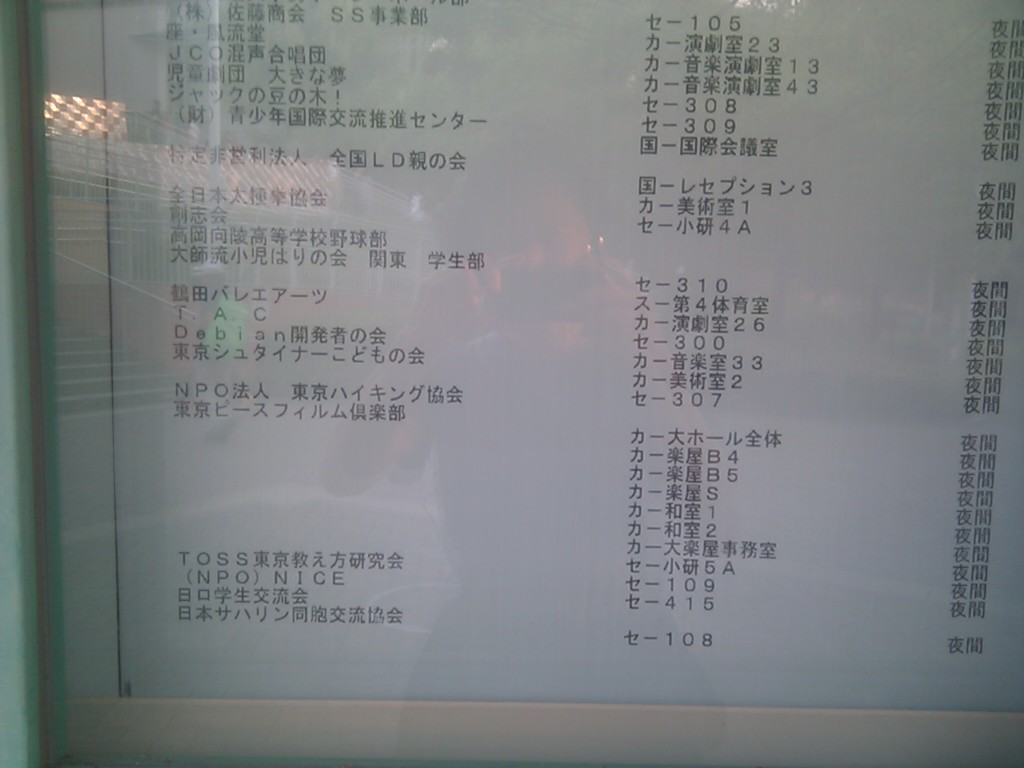
\includegraphics[width=8cm]{image201007/debianmeeting1.jpg}
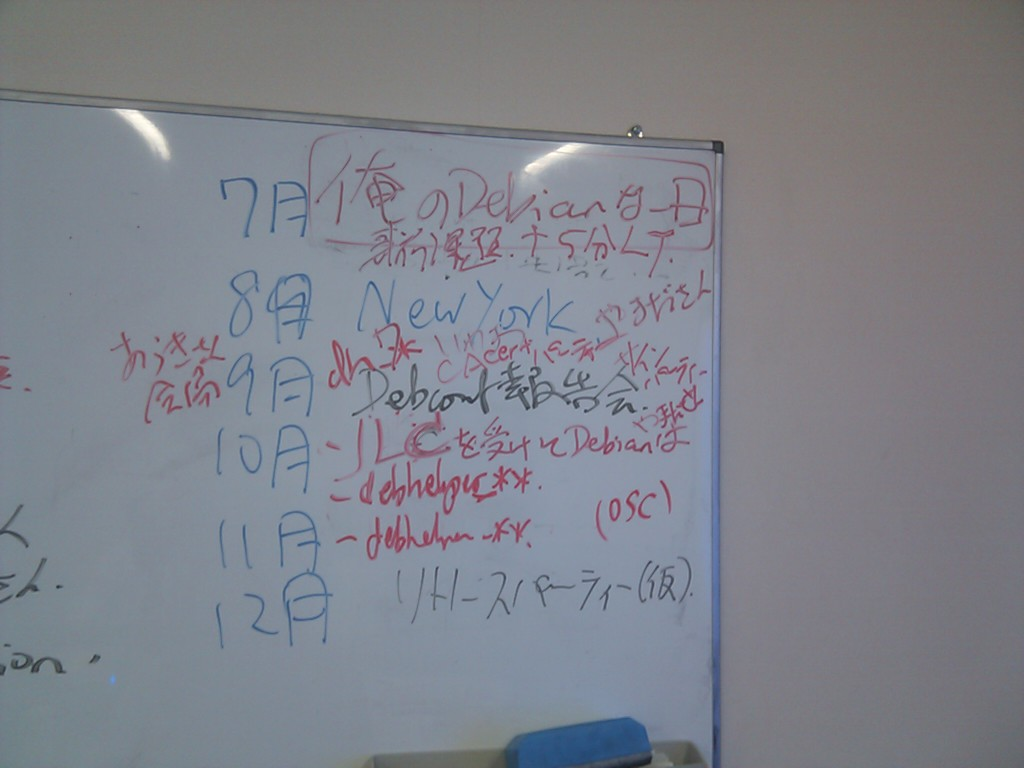
\includegraphics[width=8cm]{image201007/debianmeeting2.jpg}

%-------------------------------------------------------------------------------
\dancersection{OSC北海道参加報告}{荒木靖宏}
%-------------------------------------------------------------------------------
\index{OSC-Do 2010}


荒木の発表は「あなたはどっち、CloudでDebian, DebianでCloud」という題でDebianでのCloudにまつわる話をしました。

岩松の発表は「squeezeに向けたDebian GNU/kFreeBSD入門」という題でDebian GNU/kFreeBSDがどのようにDebianにはいり、どのように使用するのか、などの話をしました。

土曜日の朝最初のセッションで出足を心配したのですが、割り当てられた部屋はほぼ満員でした。

また、GPGキーサインパーティには事前に6人の参加表明があり、飛び入りもあり、合計8名でした。

%-------------------------------------------------------------------------------
\dancersection{Debian Conference 2010参加報告}{やまねひでき}
\label{sec:debconfreportsummary}
\index{DebConf2010}
\index{DebConf}

\subsection{DebConfとは}
年一回世界中のDebian開発者と関係者が集まって開かれるテクニカルカンファレンス「Debian Conference」のことです。
通常顔をあわせることのないメンバーたちが世界各地から一同に介し友好を深め、技術的な議論を戦わせます。

\subsubsection{Debconfの歴史・経緯}
過去の開催履歴を見てみると\tbref{tab:debconflist}のようになります。

\begin{table}[H]
\caption{歴代のDebconf参加者推移}
\label{tab:debconflist}
 \begin{center}
 {\footnotesize
 \begin{tabular}{|c|c|c|r|}
 \hline
 年 & 名前 & 場所 & 参加人数 \\
 \hline
 2000 & debconf 0 &フランス ボルドー & \\
 2001 & debconf 1 &フランス ボルドー & \\
 2002 & debconf 2 &カナダ トロント & 90名 \\
 2003 & debconf 3 &ノルウェー オスロ & 140名 \\
 2004 & debconf 4 &ブラジル ポルトアレグレ &  150名 \\
 2005 & debconf 5 &フィンランド ヘルシンキ & 200名 \\
 2006 & debconf 6 &メキシコ オアスタペック & 300名 \\
 2007 & debconf 7 &英国スコットランド エジンバラ & 約400名 \\
 2008 & debconf 8 &アルゼンチン マルデルプラタ & 約200名 \\               
 2009 & debconf 9 &スペイン エクストラマドゥーラ & 約250名 \\
 2010 & debconf 10 &アメリカ ニューヨーク & 約350名 \\
 2011 & debconf 11 &ボスニア・ヘルツェゴビナ バニャ・ルカ & ?名\\
 \hline
 \end{tabular}
 }
 \end{center}
\end{table}

\subsubsection{Debconf 2010}
今年のDebConf、DebConf10 (\url{http://debconf10.debconf.org/}) はアメリカ・ニューヨークのコロンビア大学で開催されました。
日本からは、岩松 信洋、鈴木 崇文、やまねひできの3名が参加しました。

\subsubsection{会場}
コロンビア大学キャンパスにカンファレンス会場としてトークルームに2室、BOFルームに1室、AdHocセッション用に1室、それから昼夜を問わずに作業する人のためのハックラボが2室設けられました。NYCという大都会の大学キャンパス(すぐ側に24時間運転の地下鉄駅がある)での開催ということもあり、会場周りは昼夜を問わずかなり賑やかな状態でした。ニューヨークと言うと危険なイメージがあるようですが、怖いのは街中を歩いてもものすごく体格のいい人が多いこととタトゥーな人が多いことぐらいです。

今回のネットワークは、コロンビア大学の屈強なバックボーンへGuruPlugなども使った即席手作り感満載のネットワークが接続されてました。無線が非常に繋がりにくいのなんのって…。また、Debianのミラーサーバについては、前年のスペインではDNSを乗っ取ってローカルのミラーを見せるようにしていたようですが、今回はコロンビア大学のネットワークを利用している為にそういう訳にもいかず、cdn.debian.netを使うのはどう?→ディレクトリ構成が違うからコロンビア大学は加えられない→変えたよ!→cdnに追加したよ!という感じで最終的にcdn.debian.netの改善に繋がったりしました。この後も色々とcdn.debian.netには要望が出たり、Debian Live の標準 apt line に加えられていたりといい感じでした。荒木さんに拍手。

\subsection{スケジュールとイベント}
今回は8月1日から7日が開催期間で、間の1日が Day Trip として Coney Island というニューヨークの端のビーチでのんびり&マイナーリーグの観戦という形でした。例によってDebConf期間の前に1週間 DebCamp という開発合宿も開かれていたようです。

今回イベントとして「RCBC(release critical bugs contest、\url{http://wiki.debconf.org/wiki/DebConf10/RCBC})」と題し、皆でRC(Release Critical)バグを潰そう、というものが開かれました。これによって100個以上のバグが一気に修正され、多くのバグを潰した人には懸賞としてGuruPlugやHPのelite bookやネットブック、書籍類などが進呈されていました。この期間中に岩松さんが3個、私は1個潰しましたので書籍を頂きました。でも英語なんですよね…。

\subsection{セッション}

今年は大きくトラックカテゴリとして「コミュニティ」「Java」「サイエンス」「エンタープライズ」「メディア&アート」が設けられ、それぞれに合わせたセッションが開催されました。で、肝心の内容ですが、これを書く時間が無い&もうSoftware Design 2010年10月号で書いた&ウェブから大半のセッションが見れますよ、なので SD とウェブで見てください…。サイトは \url{http://www.debianart.org/live/} です。

Debian が多くの派生ディストロの「Hub」として振る舞うことを意識した話で「Derivatives Front Desk」を設けて派生ディスリビューション間での交流を進めていくことや、特に Canonical サイドからなるべく Debian にフィードバックしようという話が盛んに出ていたことが印象に残ります。Canonical としては自前で変更点を保持していくのがコスト高なのが懸念点なのでしょう(Nexenta も Solaris 対応のパッチ維持が大変なので、という発言をしていました)。

それから Stable に対する見直しの話が出ています。安定版をより使いやすいものにするために方針を緩めて「BTS上でimportant以上のバグ修正」「FTBFS(failed to build from source, ソースからビルドができない問題)の修正」「セキュリティ勧告がでていない致命的ではないがセキュリティ上の修正」をポイントリリースで取り入れていくそうです。

\subsection{次回のDebconf}
来年はボスニアのバニャルカが開催地です。政府の全面バックアップがあるようなので Free Beer に期待。

%-------------------------------------------------------------------------------
\dancersection{OSC Tokyo 2010/Fall 参加報告}{まえだこうへい}
%-------------------------------------------------------------------------------
\index{OSC Tokyo 2010/Fall}

2010年9月11日(土)に、OSC Tokyo
2010/Fall\footnote{\url{http://www.ospn.jp/osc2010-fall/}}が春と同じく明
星大学にて開催されました。今回は、セッション2つとブース展示です。

セッションは
\begin{itemize}
 \item GPGキーサイン説明およびGPGキーサインパーティ
       \footnote{\url{http://www.ospn.jp/osc2010-fall/modules/eguide/event.php?eid=47}}
 \item でびあん らんだむとぴっくす
       \footnote{\url{http://www.ospn.jp/osc2010-fall/modules/eguide/event.php?eid=9}}
\end{itemize}
で、前者は岩松さんが、後者はやまねさんが発表を行いました。

GPGキーサインパーティには岩松さんを含め10名の参加\footnote{事前登録は12
名。}があり、GPGキーサインの説明の後、その場でキーサインが行われました。
キーサイン自体が初めての方も半数くらいいて、参加者のうち大半はその後ブー
スにも立ち寄ってくれました。

らんだむとぴっくすは、Debian 17執念、Debconf10、Squeezeの話でした。参加
者は20名を超えて、資料は文字がほとんどなく、後から資料だけを見ると大抵さっ
ぱりと思われる内容ですが、こちらも盛況でした。

ブースでは、Debian関連の書籍と、Squeeze on OpenBlockS 600の展示、Debian
へのコメントを一言、を行いました。一言もらった方にはぐるぐるステッカーを
無償で差し上げる、という試みを行いました。またDebianではなくUbuntuしか使っ
たことが無いですが何か?という人がかなり多かったのですが、そういう人に対
してはUbuntuに対する意見でも構わない、ということを伝えたのでコメント記入
の敷居が多少下がったようでした。

終了後、やまねさん、山本さん、まえだの三名で高幡不動のとんかつ和幸で打ち
上げ&反省会を、その後タリーズに移動して、Miniconfの開催についてのディス
カッションを行いました。\footnote{今回のネタにリンクする、というわけです。}

%-------------------------------------------------------------------------------
\dancersection{LinuxCon Japan 2010 参加報告}{鈴木崇文}
%-------------------------------------------------------------------------------
\index{JLC}

LinuxCon Japan 2010は9月27~29日の日程で六本木アカデミーヒルズで開催され
ました。参加したセッションは主に次の二つです。
\begin{itemize}
 \item MeeGo
 \item Samba
\end{itemize}
また、同日開催されたCELF BoFについて、Ubuntu絡みの話について聞いてきたの
で、セッションの内容について、および、今回のLinuxConの規模、参加者、その
場の雰囲気について、今回の勉強会で報告します。

%-------------------------------------------------------------------------------
\dancersection{あるDebianな一日}{上川純一}
%-------------------------------------------------------------------------------

\subsection{始まり}

朝起きる、ワシントンDCで買ってきたスターバックスのマグカップに湯を注ぎコ
コアをいれる。まだ外は暗い。おもむろにマシンを起動する。SSDベース
\footnote{内蔵ディスクがHDDではなくてSSDのモデルがある。}のvaio
type Pはしずかに起動する。grub はLinux パーティションを自動起動するように設
定されており、ひとしきりLinuxの起動メッセージが画面に流れたあとGDのログ
イン画面が登場する。
ユーザ名とパスワードを入力。画面はきりかわり、いくつか
のアプリケーションが自動で起動する。
pidgin, google-chrome, emacs 22, gnome-terminal。
\index{pidgin}
\index{google-chrome}
\index{emacs}
\index{gnome-terminal}

毎日ではない、でも週に一回はこの日がくる。
今日はバックアップをとる。USB経由で接続できる 2.5インチ
ディスクを接続し、ディスクがスピンアップするのを待つ。
backup.sh を実行するとLVM ボリュームのスキャン、ext3 ファイルシステムのマウントと
\texttt{pdumpfs} の実行処理がはしり、かりかりとバックアップがとられる。
定期的なバックアップ作業の一環として、ディスクの使用量を確認する。\texttt{df -i} で inode の残量、 \texttt{df -h} でディスク容量
の残量を確認する。まだ余裕があるようだ。
\index{pdumpfs}
\index{df -i}
\index{df -h}

\begin{commandline}
$ df -i 
/dev/mapper/vgvaio-vaiohome
                     5242880  417994 4824886    8% /home
/dev/mapper/vgusb1-coreduohome
                     4587520 1116140 3471380   25% /mnt
$ df -h 
/dev/mapper/vgvaio-vaiohome
                       79G   64G   12G  85% /home
/dev/mapper/vgusb1-coreduohome
                       69G   46G   21G  70% /mnt

\end{commandline}

メールを取り込む。メールはssh経由の独自のバッチプロトコルで取得する。
これは高レイテンシネットワーク(Air H'') をつかっ
ていた時代からの名残りだ。
そして \texttt{M-x wl} で wanderlust を立ち上げる。
\index{wanderlust}

\subsection{開発環境のメンテナンス}

開発環境をメンテナンスする。

まず、パッケージを最新にする。 apt-get update, apt-get upgrade, apt-get
dist-upgrade を行う。手元の環境はときによりstableだったりtesting だったりする。最
近はvaio type Pではstableを使っている。

開発用につかっている chroot イメージをアップデートする。
\texttt{cowbuilder --update} で最新のパッケージをダウンロードしていくる。
chroot環境はsidを基本としている。

あと他にもchroot環境がいくつかあったりする。
cowbuilder ではない環境も用意してある。\texttt{/home}をバインドマウント
している chroot ディレクトリがあり、\verb!chroot_sid.sh!コマンドで
その環境に入れるようにしてある。自作の jchroot コマンドを使い
現在の実行しているユーザ、現在のディレクトリと同じ場所、でchroot内部の
bashが立ち上がるようになっている。標準のchroot コマンドだけだといまいち
かゆいところに手が届かないのと、dchrootコマンドの実装がいまいち気に入ら
ないから自作してしまった。
\index{dchroot}
\index{jchroot}
\index{cowbuilder}

手元の apt ミラーとして approx が動いているので、同じパッケージを複数の
chroot 環境で必要となっても大丈夫だ。
\index{approx}

\subsection{バグレポートの処理}

パッケージのメンテナンスをする、主となるのはバグレポートの対応だ。
バグレポートは\url{http://bugs.debian.org/}のウェブインタフェースで確認
できる。
手元で欲使うのはメールインタフェースだ。
バグ報告はメールとして送られてくる。

emacs をたちあげ、 wanderlust を立ち上げる。
バグレポートにパッチが添付されていれば、それを適用する。
手順としては、 ``e'' でメールをファイルとして保存し、
そのファイルをソースコードのディレクトリに移動して git am で適用する。
今日はpbuilder のバグ処理をしているので、pbuilder のソースツリーのディレ
クトリに移動し順にパッチを適用していく。

残念ながらこの一番シンプルなフローにしたがってくれるバグ報告は少ない.
ほとんどのバグ報告ははパッチつきではないし、ついていたとしても手直しなし
で適用できるものではない。
そういう場合はいろいろといじってから \texttt{git commit} することになる。

\subsection{テストとリリース}

パッケージをビルドしてテストするスクリプトは自動化している。emacs lisp で
書いてあり、emacs からビルドとテストが実行されるようになっている。
\texttt{cowbuilder --build} を実行して、すべて成功したら日付別になっている「成功し
たファイル置き場」においてくれるというもの。

管理しているパッケージはすべて \texttt{debian/pbuilder-test/} ディレクトリにテスト
スクリプトがあり、そのスクリプト全部が正常に実行できれば基本的な動作はで
きていると考える。
メンテナンスのコストを軽減するためにはテスト重要。

正常な動作をするパッケージが生成できるソースコードが準備できたら、
\texttt{denbian/changelog}を整備する。
まず、git dch -a でchangelog の雛形を生成して、編集。
debian-changelog modeをつかって、 \texttt{C-c C-e C-c C-d unstable C-c C-c}.

\texttt{git commit} して、 \texttt{git-tag.sh}というスクリプトを使って署名つきのタグを作成。
前出のelispを使って最終版のパッケージをcowdancer環境でビルドする。
\texttt{debsign} コマンドでできたパッケージに署名、その後\texttt{dput}でアップロード。

しばらく放置していると
ftp master から無事に accept されたというメールがくる。
これを受けてリポジトリの内容を \texttt{git push --tags},  \texttt{git push} する。

新しいパッケージがこれでリリースできた。

\dancersection{Mini Debconfにむけてのディスカッション}{山本浩之}
\index{Miniconf}

mini debconfを日本での開催実現に向け、ディスカッションを行います。以下を
叩き台にとして、みんなでブレストしてみましょう。

\subsection{セッション内容}
\subsubsection{前提}
基本英語でやれるように…したい。でないと、海外から招待したゲストがまったく分からん状態になる。
\subsubsection{Embedded}
\begin{itemize}
 \item 組み込み系とdistroの間の溝を埋めるようなことができないか。一から
       古いバージョンのソースをスクラッチで作っているような状況をdebian
       をつかうことで改善できるような提案ができると強い。
 \item Emdebianの取り組みを聞けたりするとうれしいか?
 \item portingについてのネタも聞きたい。
\end{itemize}

\subsubsection{Free (like Debian day)}
\begin{itemize}
 \item Free とライセンスという観点から Creative Commons とコラボレーショ
       ンはどうか\\
       「コンテンツ製作者」と「ソフトウェア製作者」は微妙に層がずれてい
       るので、自由な制作物を生み出すライセンスという観点から、ここで交
       流ができないものか。自由なコンテンツと自由なソフトウェアの交流で、
       少しでもdebianに自由なコンテンツが流入して豊かなソフトを利用者に
       提供できないか。
\end{itemize}

\subsubsection{事例集}
\begin{itemize}
 \item 利用事例を出して、CentOSではなくDebianを選択肢として考えてもら
       えないか。要は最初に何を使うかが肝。実際、RHELにするつもりで商用
       ソフトでサポートが必要ならCentOSはありだと思うが、そうでなければ
       Debianで全く問題ないはず。なのにCentOSを使う例が結構ある。
 \item 実際に使っているgreeさんとか、pixivさんとか、楽天さん?とか、朝日
       ネットさんなどから話を聞ければありがたい。
 \item これからLinuxを利用しようとする場合に実際に利用している、ある程度
       の成功を収めている例があるのは心強い。さらに優位性を説明できれば
       なおよい。
\end{itemize}

\subsubsection{言語系セッション}
需要高い?

\subsubsection{その他}
\begin{itemize}
\item derivatives セッションとかどうだろうか。
\item エストレマドゥーラの自治体の発表とか聞ければ楽しいか?
\item ライセンスセッションとかあってもいいかも。この前 java-ja でも結構
      盛り上がった。でも日本語ベースになると思われる。
\end{itemize}

\subsection{5H2H}
\subsubsection{When}
 2011年前半がいい?2010年はもう難しい。2011年後半だと時間が経ちすぎ。
\subsubsection{what}
次の2つは相互に影響しあう。何をするか(何ができるか)と、何を目的にするかは鶏と卵。
\begin{itemize}
 \item 何をするか\\
       セッションネタを考える
 \item 何を目的にするのか
       \begin{itemize}
	\item 開催した後に何が成果になるのか
	\item 誰をターゲットにするのか
	\item debianとどういうつながりにするか
	\item スポンサードしてくれるところへのメリット(ここを重要視しすぎない)
       \end{itemize}
\end{itemize}
\subsubsection{Who}
\begin{itemize}
 \item スタッフの必要人数\\
       何に何人必要?何がタスクとしてあるのかを洗い出す。
 \begin{itemize}
  \item 事務局、当日受付、機材準備、通訳
  \item 実際の例を確認する
 \end{itemize}
\end{itemize}
\subsubsection{When}
開催する内容(セッション、イベント)との兼ね合い
\subsubsection{how much}
費用はどの程度かかるのか
\begin{itemize}
 \item 招待者の旅費、宿泊費、食費
 \item 会場費
 \item ネットワーク機器、電源周り、ビデオ撮影、マイクなどの機材
\end{itemize}
\subsubsection{where}
海外から人を呼ぶならそれなりに接続が良い・移動に費用がかからない方がいい

\printindex

\cleartooddpage

\vspace*{15cm}
\hrule
\vspace{2mm}

\includegraphics[width=2cm]{image200502/openlogo-nd.eps}
\noindent \Large \bf Debian 勉強会資料\\ \\
\noindent \normalfont \debmtgyear{}年\debmtgmonth{}月\debmtgdate{}日 \hspace{5mm}  初版第1刷発行\\
\noindent \normalfont 東京エリア Debian 勉強会 (編集・印刷・発行)\\
\hrule

\end{document}
